

\chapter{Planificación}

\section{Planificación temporal}

\subsection{Fases del proyecto}

En este apartado se mencionan cada una de las fases en las que se pretende dividir el desarrollo del proyecto. Con cada fase se incluye una explicación de los temas a desarrollar. En el siguiente apartado de la sección se encuentra el \textit{diagrama de Gantt} correspondiente.

\subsubsection{Fase inicial o de investigación}

En cuanto a la primera fase del desarrollo del proyecto, se comenzará con una investigación teórica sobre lo que es el trading, trading algorítmico y demás conceptos de economía que entren en juego en el tema. Aquí se realizará también una investigación sobre dos de los principales referentes del análisis de mercados: \textit{Charles Dow} y \textit{Richard Wyckoff}. \newline

En esta fase también se harán programas de ejemplo usando las distintas \textit{APIs} de conocidas plataformas de trading como son \textit{MetaTrader} o \textit{Binance} (específica para criptomonedas). \newline

Durante este período también se estudiarán las posibles herramientas a usar para el proyecto. Se seguirán tutoriales de \textit{Django} ya que se decidió que la APP fuera implementada usando este framework y por tanto, programada con \textit{Python}. También se estudiará la viabilidad de realizar el proyecto en \textit{Windows}, ya que librerías como la de \textit{MetaTrader5} para \textit{Python} sólo están disponibles en este sistema operativo. \newline


Podemos llamar a esta fase inicial o de investigación y se pretende que sea la que más tiempo ocupe en el desarrollo del proyecto debido a que tener bases sólidas sobre el tema es vital para el transcurso del trabajo. Se prevee que ocurra desde la propuesta del proyecto, noviembre de 2020, hasta principios de 2021. \newline


\subsubsection{Fase de recopilación de datos}

En esta segunda fase de desarrollo del proyecto se pretende investigar qué volumen de datos históricos de mercados financieros podríamos recopilar de internet u otras fuentes. Esta acción es necesaria previa al análisis de lo que va a ser el producto software, ya que en todo caso, se necesitará cierto volumen de datos para poner a funcionar los algoritmos de trading, ya fuesen de análisis puro, o de aprendizaje automático. \newline

En la primera aproximación, se implementarán una serie de scripts en \textit{Python} para obtener datos de mercados a través de \textit{MT5}. Con estos scripts, se busca conseguir el mayor volumen de datos posible para el mayor número de mercados financieros posibles. \newline

Debido a la clara limitación en espacio que esto supone se estudiará la posiblidad limitar el número de mercados financieros a tratar, buscando diversidad en cuanto a tener varios tipos de mercados. \newline

Esta fase de recopilación de datos históricos supondría desde principios de 2021 hasta principios del Q2 (abril-mayo) de 2021.

\subsubsection{Fase de análisis}

En la fase de análisis, se realizará la especificación de requisitos funcionales, no funcionales y de información. En esta fase también se describirán los implicados en la aplicación. \newline

Esta fase ocurrirá justo al finalizar la etapa anterior y no durará más de dos o tres semanas.

\subsubsection{Fase de diseño}

En la cuarta fase del desarrollo del proyecto, se propondrá el diseño a alto nivel de la aplicación. En esta fase de diseño, se estudiará la arquitectura del software a desarrollar con un diagrama de paquetes o módulos en los que se dividirá la aplicación. \newline

En este punto se presentará también el primer boceto de diseño de la interfaz presente en la aplicación web. \newline

Esta fase ocupará dos semanas más y ocurrirá inmediatamente después de la fase de análisis.

\subsubsection{Fase de desarrollo}

En la fase de desarrollo de código del proyecto es donde se comenzará con la implementación del producto software. \newline

Este período se describirá de manera más detallada en el capítulo \ref{cap:implementacion}. En dicho capítulo se explicará la metodología ágil usada para el seguimiento del desarrollo y cada una de las issues de \textit{GitHub} creadas para implementar la aplicación. \newline

Esta fase se desarrollará desde junio hasta la tercera semana de agosto de 2021.

\subsubsection{Fase de pruebas}

La última parte del proyecto recae en una fase de pruebas. En esta fase se realizarán pruebas y se incluirán posibles fixes de última hora para bugs encontrados. Esta fase también servirá como retroalimentación para las conclusiones y para ver algunos resultados del algoritmo en funcionamiento. \newline


Este último período del proyecto ocurrirá en la última semana de agosto y primera de septiembre de 2021.

\subsection{Diagrama de Gantt}

En la figura \ref{diagrama_gantt} se muestra el diagrama de Gantt correspondiente con las fases del proyecto anteriormente mencionadas. \newline


\begin{sidewaysfigure}[!h]
	\centering
	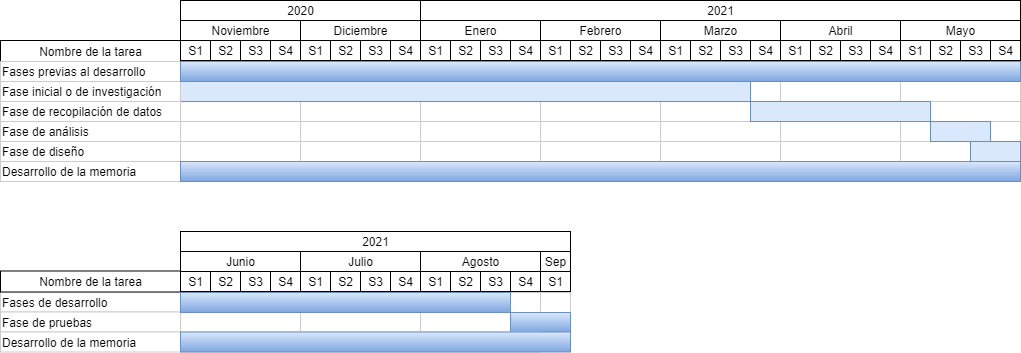
\includegraphics[width=\textwidth]{imagenes/gantt.png}
	\caption{Diagrama de \textit{Gantt} del proyecto} \label{diagrama_gantt}
\end{sidewaysfigure}



\section{Presupuesto de ejecución}

En este apartado menciono una aproximación de los posibles costes del desarrollo del proyecto. Detallo aquí los gastos por personal, equipos o recursos informáficos, licencias de softwares, etc.\newline

\subsection{Gastos de personal}

En esta sección se recoge el gasto total referente a pago de personal que ha estado trabajando en el desarrollo del proyecto. \newline

El trabajo ha sido realizado por un grupo de una sola persona o desarrollador con tutorías de un profesor. \newline

Suponiendo que dicha persona es recién egresada, su puesto sería el de desarrollador Junior. Si echamos un ojo a páginas web externas que proporcionan datos como la media de sueldos por trabajo y ciudad, vemos que el salario base promedio de un programador Junior en Granada a tiempo completo es de 16.432 \euro/año, lo que sería equivalente a un total de 1.163 \euro/mes. Fuente: \color{blue}\href{https://es.indeed.com/career/programador-junior/salaries/Granada--Granada-provincia}{https://es.indeed.com/career/programador-junior/salaries/Granada--Granada-provincia}\color{black}.\newline

Viendo el diagrama de Gantt descrito en el anterior punto de la memoria, preveemos que el desarrollo del proyecto dure 10 meses. Suponiendo que el trabajador trabajará a media jornada (4 horas diarias, suponiendo un total aproximado de 400 horas), el pago total que se le haría sería de 1.163 * 10 / 2 = 5.815 \euro.\newline

A esto hay que sumarle las horas invertidas por el tutor del proyecto en las entrevistas y seguimiento de la aplicación. Aproximando el número de entrevistas previstas a 4 en la fase de investigación y 6 en la fase de desarrollo; y suponiendo una duración de 1 hora por entrevista y coste de 35 \euro/entrevista, tendremos una inversión de 350 \euro.\newline

\subsection{Gastos de recursos informáticos y energía}

En este apartado se recoge el gasto referente a la obtención de recursos informáticos, tanto de hardware como de software necesario para el desarrollo del proyecto, así como gastos referentes a licencias y software.\newline

\begin{itemize}
	\item \textbf{Equipo usado para el desarrollo del proyecto:} Lenovo Legion 5 - Portátil Gaming 15.6" FullHD 144Hz (AMD Ryzen 7 4800H, 16GB RAM, 512GB SSD, Nvidia RTX2060-6GB, Windows 10). \\ \textbf{Coste: 999 \euro}\newline
	\item \textbf{Periféricos adicionales:} Monitor extra, ratón y teclado.\\ \textbf{Coste: 200 \euro}\newline
	\item \textbf{Licencia del IDE de desarrollo previsto, PyCharm}: Se prevee que se pueda hacer un uso gratuito del mismo, pero se contemplará la posibilidad de usar su versión Professional. Licencia gratuita con correo institucional de la universidad pero que a priori es de pago.\\ \textbf{Coste: 8,90 \euro/mes = 89 \euro}\newline
	\item \textbf{Resto de software:} El resto de aplicaciones y licencias que se preveen usar son de uso gratuito.\newline
\end{itemize}

Además de los recursos informáticos, recogemos en este apartado el gasto energético supuesto en el desarrollo del trabajo. Asumiendo que se trabajará durante 10 meses a media jornada y suponiendo el gasto medio actual en españa al mes (40 \euro) en lo que a electricidad se refiere, dicho gasto ascenderá a un total de 400 \euro.\newline

\subsection{Resumen del presupuesto}

En la figura \ref{presupuesto} se resumen todos los gastos vistos en las secciones anteriores. \newline

\begin{figure}[h]
	\begin{center}
		\begin{tabular}{| c | c |}
			\hline
			\multicolumn{2}{ |c| }{\cellcolor{blue!25}Presupuesto} \\ \hline
			Total sueldos desarrollador Junior & 5.815 \euro \\ \hline
			Horas de seguimiento &  350 \euro \\ \hline
			Equipo & 1199 \euro \\ \hline
			Licencias de software & 89 \euro \\  \hline
			Electricidad & 400 \euro \\ \hline \hline
			Total gastos previstos & 7.853 \euro \\ \hline
			
		\end{tabular}
		\caption{Presupuesto de ejecución del trabajo}  \label{presupuesto}
	\end{center}
\end{figure}